\section{McCulloch-Pitts-Neuron}

Im Jahr 1943 entwickelten Warren McCulloch und Walter Pitts ein Modell welches die Funktionalität eines biologischen Neurons imitieren sollte. In der folgenden Abbildung \ref{fig:bioNeuron} ist der grobe Aufbau eines Neurons zu sehen. 

\begin{figure}[!htb]
	\centering
	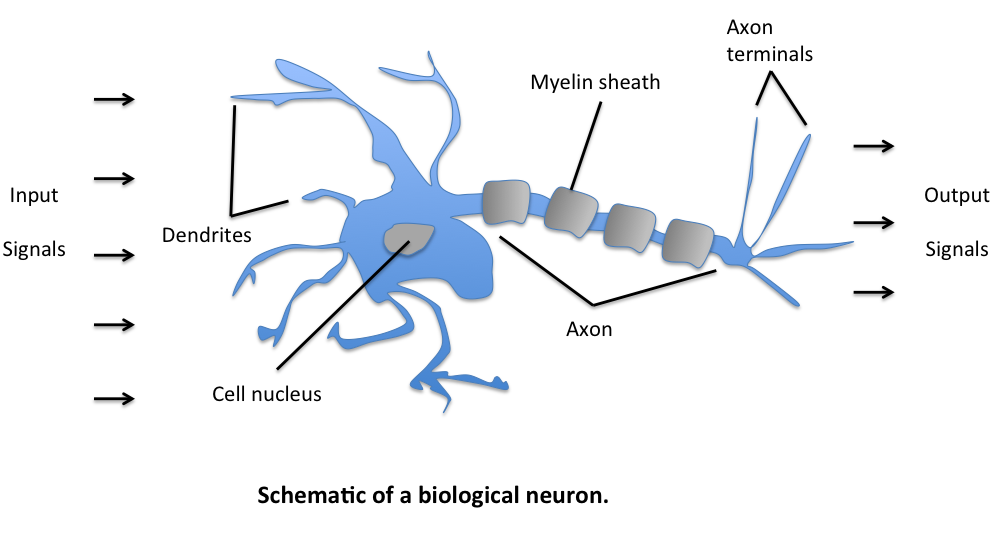
\includegraphics[width=\linewidth]{img/bioNeuron}
	\caption{McCulloch-Pitts-Zelle - Genereller Aufbau \cite{mpNeuron} \cite{perceptronAdeline}}
	\label{fig:bioNeuron}
\end{figure}

Die sogenannten \emph{Dendriten} (englisch \emph{dendrites}) nehmen Informationen auf. Sie besitzen Rezeptoren welche in der Lage sind Signale anderer Neuronen aufzunehmen. Diese Signale bewirken elektrische Veränderungen in dem Neuron welche vom Zellkörper (\emph{Soma}) interpretiert / verarbeitet werden. Dieser Zellkörper sammelt alle Informationen und speichert diese im sogenannten \emph{Axonhügel} (engl. Axonhillock) welcher die Ursprungsstelle des \emph{Axons} beziehungsweise \emph{Neuriten} beschreibt. Wenn das gebündelte Signal stark genug sein sollte wird es an den nächsten Teil des Neurons, dem \emph{Axon}, weitergeleitet. Ab diesem Zeitpunkt wird das Signal als \emph{Aktionspotential} bezeichnet und wird über die \emph{Axon} übertragen. Am Ende wird das Signal an diverse \emph{Axonterminale} weitergeleitet welche per Neurotransmitter mit den jeweils nächsten Dendriten verbunden sind. 

Dieser biologische Aufbau dient als Grundlage für die Entwicklung des Modells von McCulloch und Pitts. Das Augenmerk ihres Modells liegt in erster Linie darauf logische Gatter mittels eines Neuronen ähnlichen Modells zu definieren. Der grobe Aufbau eines sogenannten \emph{McCulloch-Pitts-Zelle} ist in \ref{fig:mpn_aufbau} zu sehen. 


\begin{figure}[!htb]
	\centering
	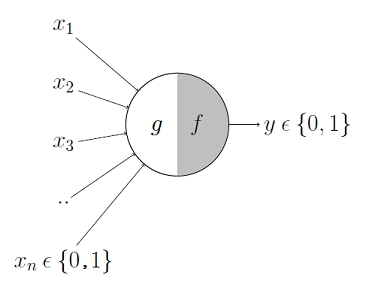
\includegraphics[width=.5\linewidth]{img/aufbau}
	\caption{Biologische Neuronen - Genereller Aufbau \cite{mpNeuron}}
	\label{fig:mpn_aufbau}
\end{figure}

Das Modell kann beliebig viele Input-werte aufweisen. Wichtig hierbei: Sie dürfen nur boolescher Natur sein (nur falsch oder wahr). Bei gegebenen Werten führt das Neuron selbst zwei Arbeitsschritte durch: 
\begin{enumerate}

\item Erst werden alle Werte aufaddiert (in der Abbildung dargestellt durch die Funktion \emph{g}). Dies imitiert das Verhalten der \emph{Dendriten} in einem biologischen Neuron. 

\item Anschließend überprüft die Funktion \emph{f} ob ein gegebener Schwellwert überschritten wurde oder nicht (gibt dies entsprechend in Form einer booleschen Ausgabe weiter). Das biologische Neuron tut dies mittels des \emph{Axonhügels}. 

\end{enumerate}

Die übliche Notation dieses Modells gibt vor, dass der jeweilige Schwellwert jeweils in die linke Seite des Kreises geschrieben wird während die rechte Seite ausgegraut wird. Im folgenden seien einmal beispielhaft das \emph{AND} und das \emph{OR} Gatter dargestellt. 

\begin{figure}[!htb]
	\centering
	\href{http://commons.wikimedia.org/wiki/File:Pachydyptes_ponderosus.jpg}{
		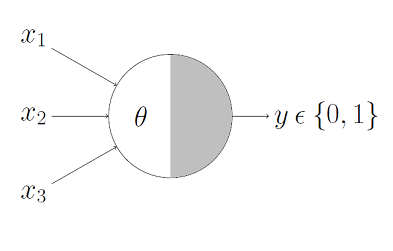
\includegraphics[width=.5\linewidth]{img/aufbau2}
	}
	\caption{Biologische Neuronen - Notation}{\cite{mpNeuron}}
	\label{fig:mpn_notation}
\end{figure}

\begin{figure}[!htb]
	\centering
	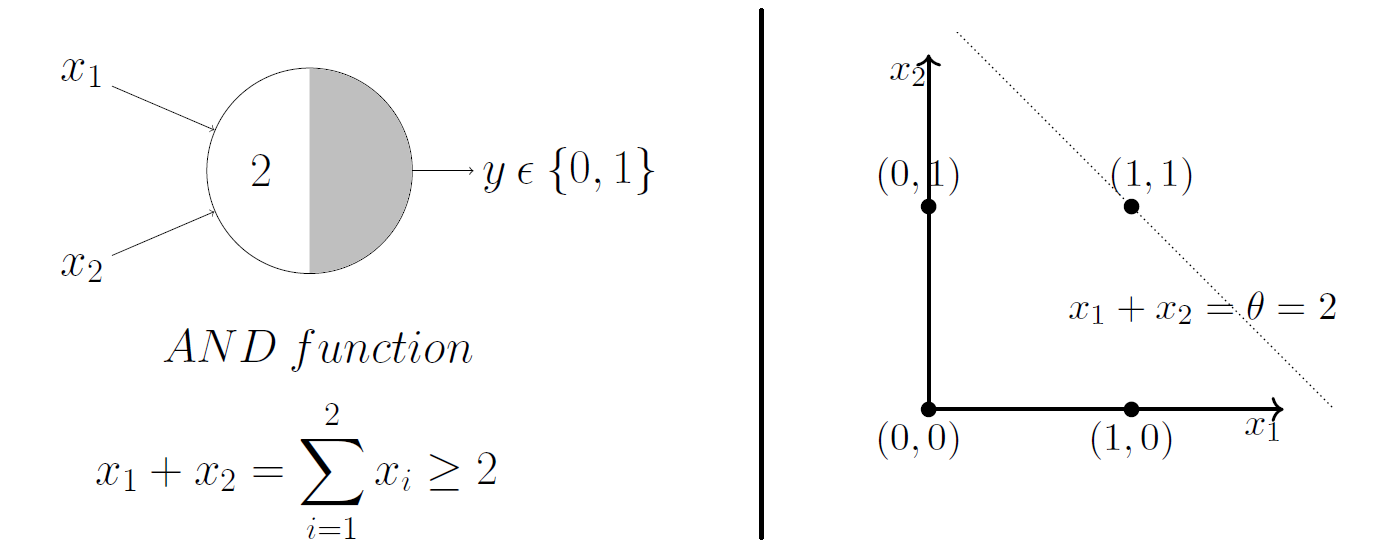
\includegraphics[width=\linewidth]{img/mpn_and}
	\caption[McCulloch-Pitts-Zelle - AND Gatter]{McCulloch-Pitts-Zelle - AND Gatter \small{Quelle \cite{mpNeuron}}}
	\label{fig:mpn_and}
\end{figure}

\begin{figure}[!htb]
	\centering
	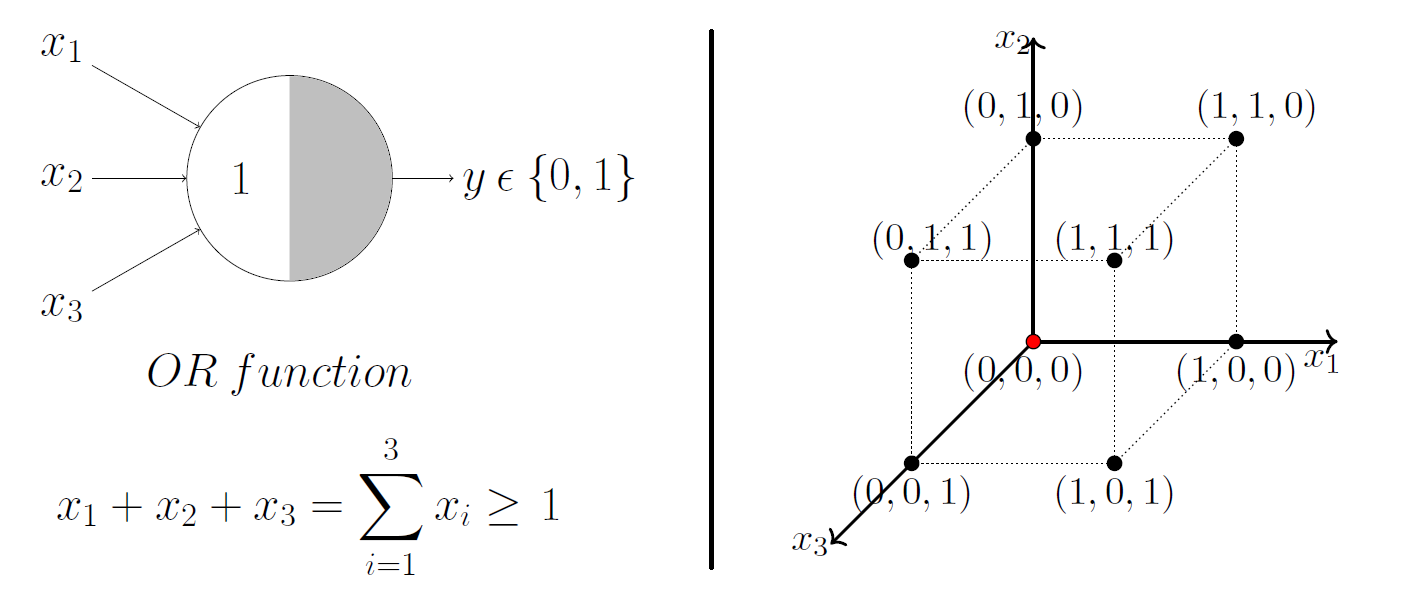
\includegraphics[width=\linewidth]{img/mpn_or}
	\caption{McCulloch-Pitts-Zelle - OR Gatter \cite{mpNeuron}}
	\label{fig:mpn_or}
\end{figure}

